\section{Signal reach}
\label{sec:signal}

In this Section we take a first look at the 
reach of this search for the T2tt and T2bw simplified models 
(Figure~\ref{fig:SigDiagram}).  Since this is a first look, not 
all the i's are dotted and not all the t's are crossed  (and the 
T2bw MC is still missing).  However, it is instructive to 
get a first feeling for where the sensitivity of this search is.
We do this in terms of ``expected limits'', assuming a null result.
The case of an excess is quite different and more complicated.

The signal efficiency in the stop vs LSP mass plane for T2tt are shown 
in Fig.~\ref{fig:SigEff}.  This figure shows clearly how difficult it
is
to have sensitivity near the kinematical boundaries.
The expected limits, under two different 
scenarios for the uncertainty on the background, are shown in
Fig.~\ref{fig:limO} and~\ref{fig:limP}.  The complementarity of the 
different signal regions is readily apparent.  
The sensitivity to low (high) stop masses comes from the 
low (high) \met\ signal regions.


\begin{figure}[hbt]
  \begin{center}
        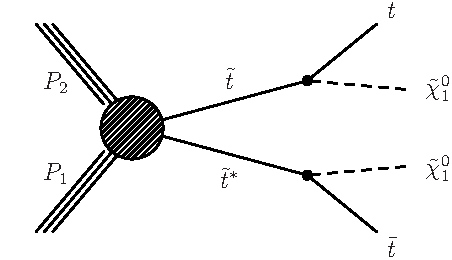
\includegraphics[width=0.5\linewidth]{plots/stopPlot/T2tt.pdf}%
        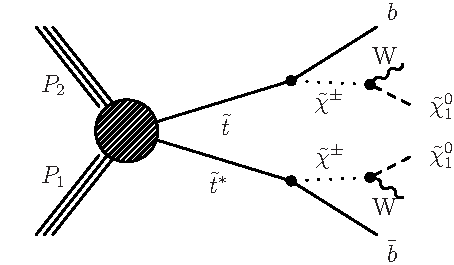
\includegraphics[width=0.5\linewidth]{plots/stopPlot/T2bw.pdf}%
	\caption{Diagram for the T2tt and T2bw simplified model.}
	\label{fig:SigDiagram}
      \end{center}
\end{figure}


\begin{figure}[hbt]
  \begin{center}
        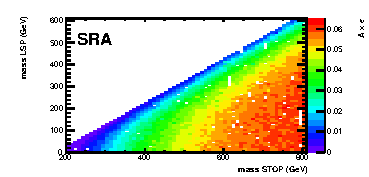
\includegraphics[width=0.5\linewidth]{plots/stopPlot/massesA_eff.pdf}%
        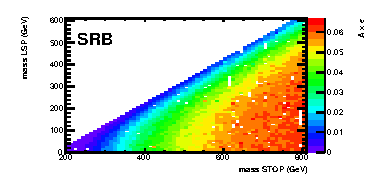
\includegraphics[width=0.5\linewidth]{plots/stopPlot/massesB_eff.pdf}
        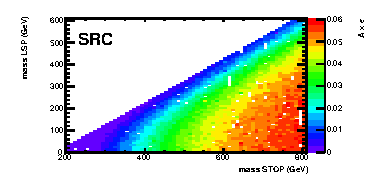
\includegraphics[width=0.5\linewidth]{plots/stopPlot/massesC_eff.pdf}%
        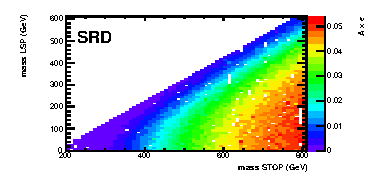
\includegraphics[width=0.5\linewidth]{plots/stopPlot/massesD_eff.pdf}
        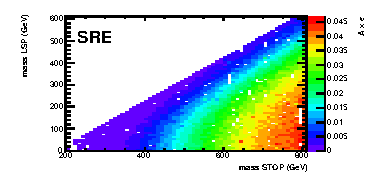
\includegraphics[width=0.5\linewidth]{plots/stopPlot/massesE_eff.pdf}%
    \caption{Signal efficiency in for the T2tt }
\label{fig:SigEff}
      \end{center}
\end{figure}

\begin{figure}[hbt]
  \begin{center}
        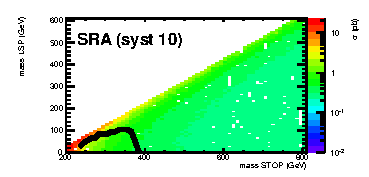
\includegraphics[width=0.5\linewidth]{plots/stopPlot/masses_SRA_xsecO.pdf}%
        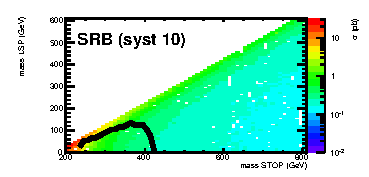
\includegraphics[width=0.5\linewidth]{plots/stopPlot/masses_SRB_xsecO.pdf}
        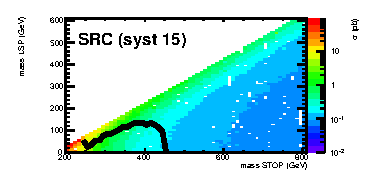
\includegraphics[width=0.5\linewidth]{plots/stopPlot/masses_SRC_xsecO.pdf}%
        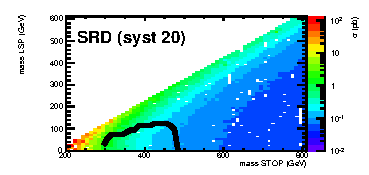
\includegraphics[width=0.5\linewidth]{plots/stopPlot/masses_SRD_xsecO.pdf}
        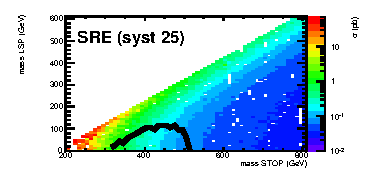
\includegraphics[width=0.5\linewidth]{plots/stopPlot/masses_SRE_xsecO.pdf}%
    \caption{Expected upper limit on the cross section for the
      T2tt. A somewhat optimistic scenario is considered as systematics on the
      background.
The assumed uncertainties on the background (in percent) is indicated on the plot.}
\label{fig:limO}
      \end{center}
\end{figure}

\begin{figure}[hbt]
  \begin{center}
        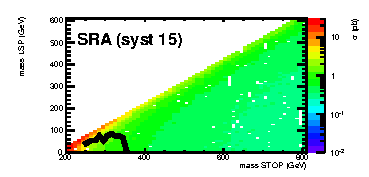
\includegraphics[width=0.5\linewidth]{plots/stopPlot/masses_SRA_xsecP.pdf}%
        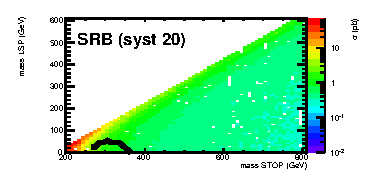
\includegraphics[width=0.5\linewidth]{plots/stopPlot/masses_SRB_xsecP.pdf}
        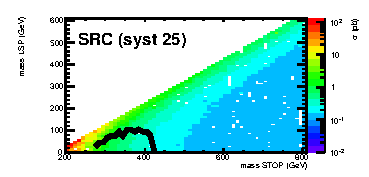
\includegraphics[width=0.5\linewidth]{plots/stopPlot/masses_SRC_xsecP.pdf}%
        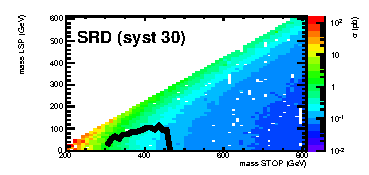
\includegraphics[width=0.5\linewidth]{plots/stopPlot/masses_SRD_xsecP.pdf}
        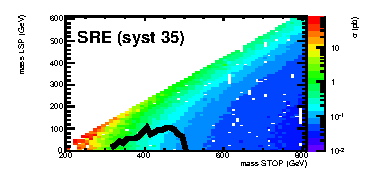
\includegraphics[width=0.5\linewidth]{plots/stopPlot/masses_SRE_xsecP.pdf}%
    \caption{Expected upper limit on the cross section for the
      T2tt. A less optimistic scenario is considered as systematics on the
      background. (compared to Fig~\ref{fig:limO}).
The assumed uncertainties on the background (in percent) is indicated on the plots.}
\label{fig:limP}
      \end{center}
\end{figure}

\clearpage
